%----------------------------------------------------------------------------
\chapter{Összefoglalás}
%----------------------------------------------------------------------------

A modellalapú szoftverfejlesztés által kínált eszközökkel világszerte a fejlesztők képesek hatékonyabban minőségibb alkalmazásokat fejleszteni. A Gamma Keretrendszer is ebben nyújt segítséget, komplex, komponens alapú rendszerek modellezését teszi lehetővé. Ennek ellenére fejlesztői környezethez való kötöttsége nehezíti a felhasználását és skálázhatóságát.

Ezen dolgozat keretein belül, egy olyan rendszert alakítottam ki, amely a felvetett problémát megoldja. A Gamma Keretrendszert átalakítottam egy olyan alkalmazás csomaggá, amely az internet segítségével bárhonnan elérhető, továbbá kötetlen és platform független, így lehetővé teszi, hogy felhőalapú megoldásként is integrálhatjuk így az ezzel járó skálázhatóságot és flexibilitást is kitudjuk használni. 
Bemutattam, hogy milyen technológiák szükségesek egy ilyen rendszer kialakításához, törekedve arra, hogy modern, korszerű megoldásokat használjak. Specifikált funkcionális és nem funkcionális követelmények alapján megterveztem a rendszer különböző komponenseit és az ezek közti kommunikációs csatornákat, majd leimplementáltam a rendszert. Az implementáció során felmerült érdekességeket és nehézségeket részleteztem és egy valós teszthalmaz segítségével teszteltem a rendszer működését.

A végső termékünk a kitűzött célnak megfelel, viszont tartalmaz olyan részeket, amelyek enyhén hiányosak vagy technikai szempontból nem optimálisak. A gamma funkciók közül mindegyik támogatott, csak a Yakindu-Gamma transzformáció nem. Az egyes fájl alapú (JSON) adattárolási megoldásokat érdemes lehet, egy adatbázissal helyettesíteni. A lejárati dátum alapú automatizált törlés implementációja jelenleg hiányos így nem működik. Egyes részekben a rendszer szinkron módon működik, érdemes lehet átgondolni, hogy az asszinkron hatékonyság a munkatér létrehozás és projekt importálás esetén releváns-e. A projekt törlés csak abban az esetben működik megfelelően ha a munkatérben nincs más projekt.

 
A \ref{specification} fejezetben leírt követelmények többségét a rendszerünk teljesíti, a pontos listát \aref{fig:requierments_placeholder_done} és \aref{fig:requierments_2_done} ábrákon lehet megtekinteni, a vastagon bekeretezett követelményeket a rendszer jelenlegi állapota teljesíti, a többi pedig részlegesen vagy egyáltalán nem teljesül.

A rendszer további fejlesztési fázisaiban meg kell vizsgálni, hogy a jelenlegi funkcionalitás kielégít-e minden felhasználói igényt, ha esetleg szükséges akkor új endpoint-ok bevezetésével egyszerűen bővíteni lehet. Az alkalmazást valamilyen konténerbe kellene helyezni, hogy a felhő integráció jelentősen egyszerűbb legyen. A felvázolt hiányosságokat a jövőben érdemes lenne áttekinteni és javítani.

A bemutatott rendszer két fontos ágazatát ötvözi az informatikának, modellalapú szoftverfejlesztés és felhőalapú alkalmazások, ezzel potenciálisan segítve a területen dolgozó mérnökök munkáját.
\begin{figure}[t]
	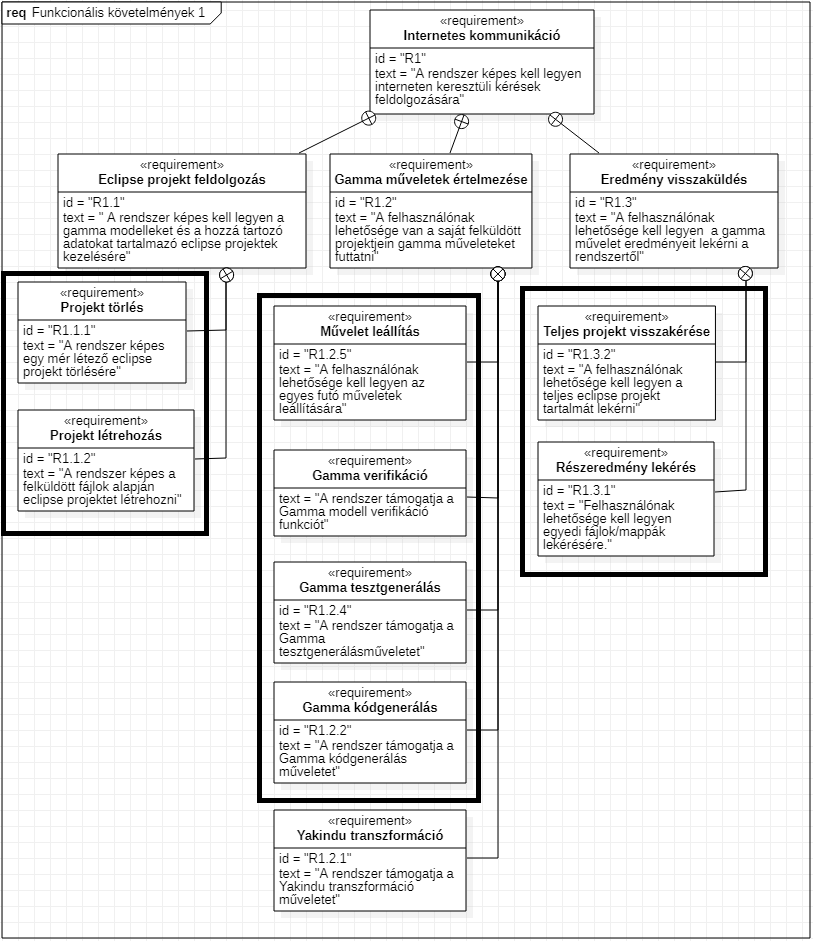
\includegraphics[width=\textwidth, keepaspectratio]{figures/requierments_placeholder_done.PNG}
	\caption{Teljesült funkcionális követelmények 1}
	\label{fig:requierments_placeholder_done}
\end{figure}
\begin{figure}[t]
	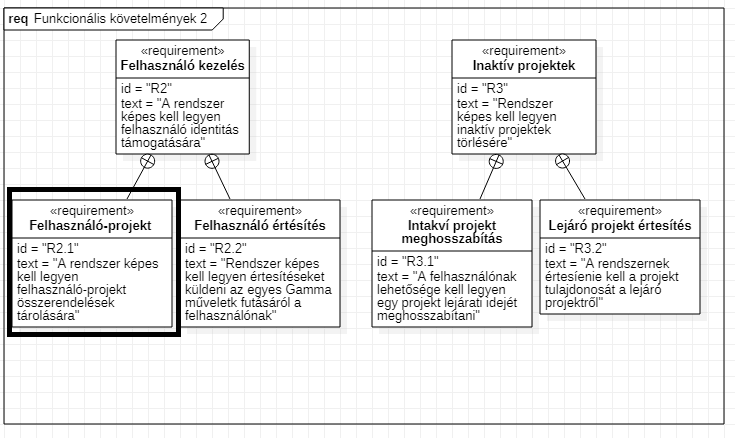
\includegraphics[width=\textwidth, keepaspectratio]{figures/requierments_2_done.PNG}
	\caption{Teljesült funkcionális követelmények 2}
	\label{fig:requierments_2_done}
\end{figure}
